\chapter{A process prediction training Framework}
\label{chap:training-framework}
During development of the models, we realized that there are highly divergent understandings regarding the batch construction for next-element predictions with sequences. We believe that this strongly impacts reproducibility of prediction approaches and present here a way that enables researchers to compare the different understandings. A selection of possible batch construction approaches is described in \autoref{sec:contrib:input-formatting}. Finally, we aim to reduce both technical understanding and reproducibility issues by providing a simple training framework in \autoref{sec:contrib:training-framework} that could be easily expanded by future researchers.

\section{Contrasts among batching strategies}
\label{sec:contrib:input-formatting}
We implemented the SP2 and PFS models as well as the comparison models using Python and the Keras neural networks API. While doing so, a wide range of recommended approaches to training the models were noted in relevant publications and on online platforms such as StackOverflow.\\

Some recommend sliding window approaches, others deem this against the concept of LSTM cells. Especially Klinkmüller et al. argue against it: "[...]the popular strategy of cutting traces to certain prefix lengths to learn prediction models for ongoing instances is prone to yield unreliable models"~\cite{klinkmuller2018reliablemonitoring}. Again others argue that padding and truncating sequences to the same length makes training faster and does not affect accuracy. Furthermore, the batch size represents an important hyper-parameter, and no guidelines how to sort traces into batches were found. We believe that the understanding of the merits of each batch construction approach is of general value to any application of sequence prediction.\\

When using Keras' implementation of LSTM, it is stateful \textit{during} a batch, and resets the internal state before the next batch~\cite{web:keras}. For the sake of simplicity, it is advisable to keep related data inside a single batch. Translated to traces, this means keeping a trace completely inside a batch. The Keras LSTM layers expect data to arrive in a three-dimensional array of fixed size for every batch, where each dimension has a defined meaning:

$$(n_{samples}, n_{timesteps}, n_{features})$$

Each sample contains a number of timesteps $n_{timesteps}$ containing a number of features $n_{features}$, which is a constant. For each sample, the LSTM layer maintains a separate state, meaning that several traces can be trained on simultaneously~\cite{web:keras-lstm-state}. As the batches themselves need not to have the same dimensions, this definition opens up a range of possible batch construction strategies, four of which we are highlighting in the following paragraphs. To the best of our knowledge, these have not been compared in this context yet.\\

First and easiest, one trace can be trained per batch. This fulfills the requirement of constant dimensions, since only a single sample is used.

Second, \textit{some} traces can be trained inside a single batch. This is possible if all traces inside one batch have the same number of timesteps, i.e. have the same length. The number of samples and timesteps may vary between batches. A look at the trace length distribution in \autoref{fig:bpic2011-length-distribution} from BPIC2011 reveals that grouped batching could bias the model toward the long tail of the distribution, as those traces are trained in batches of their own.

\begin{figure}[ht!]
    \centering
    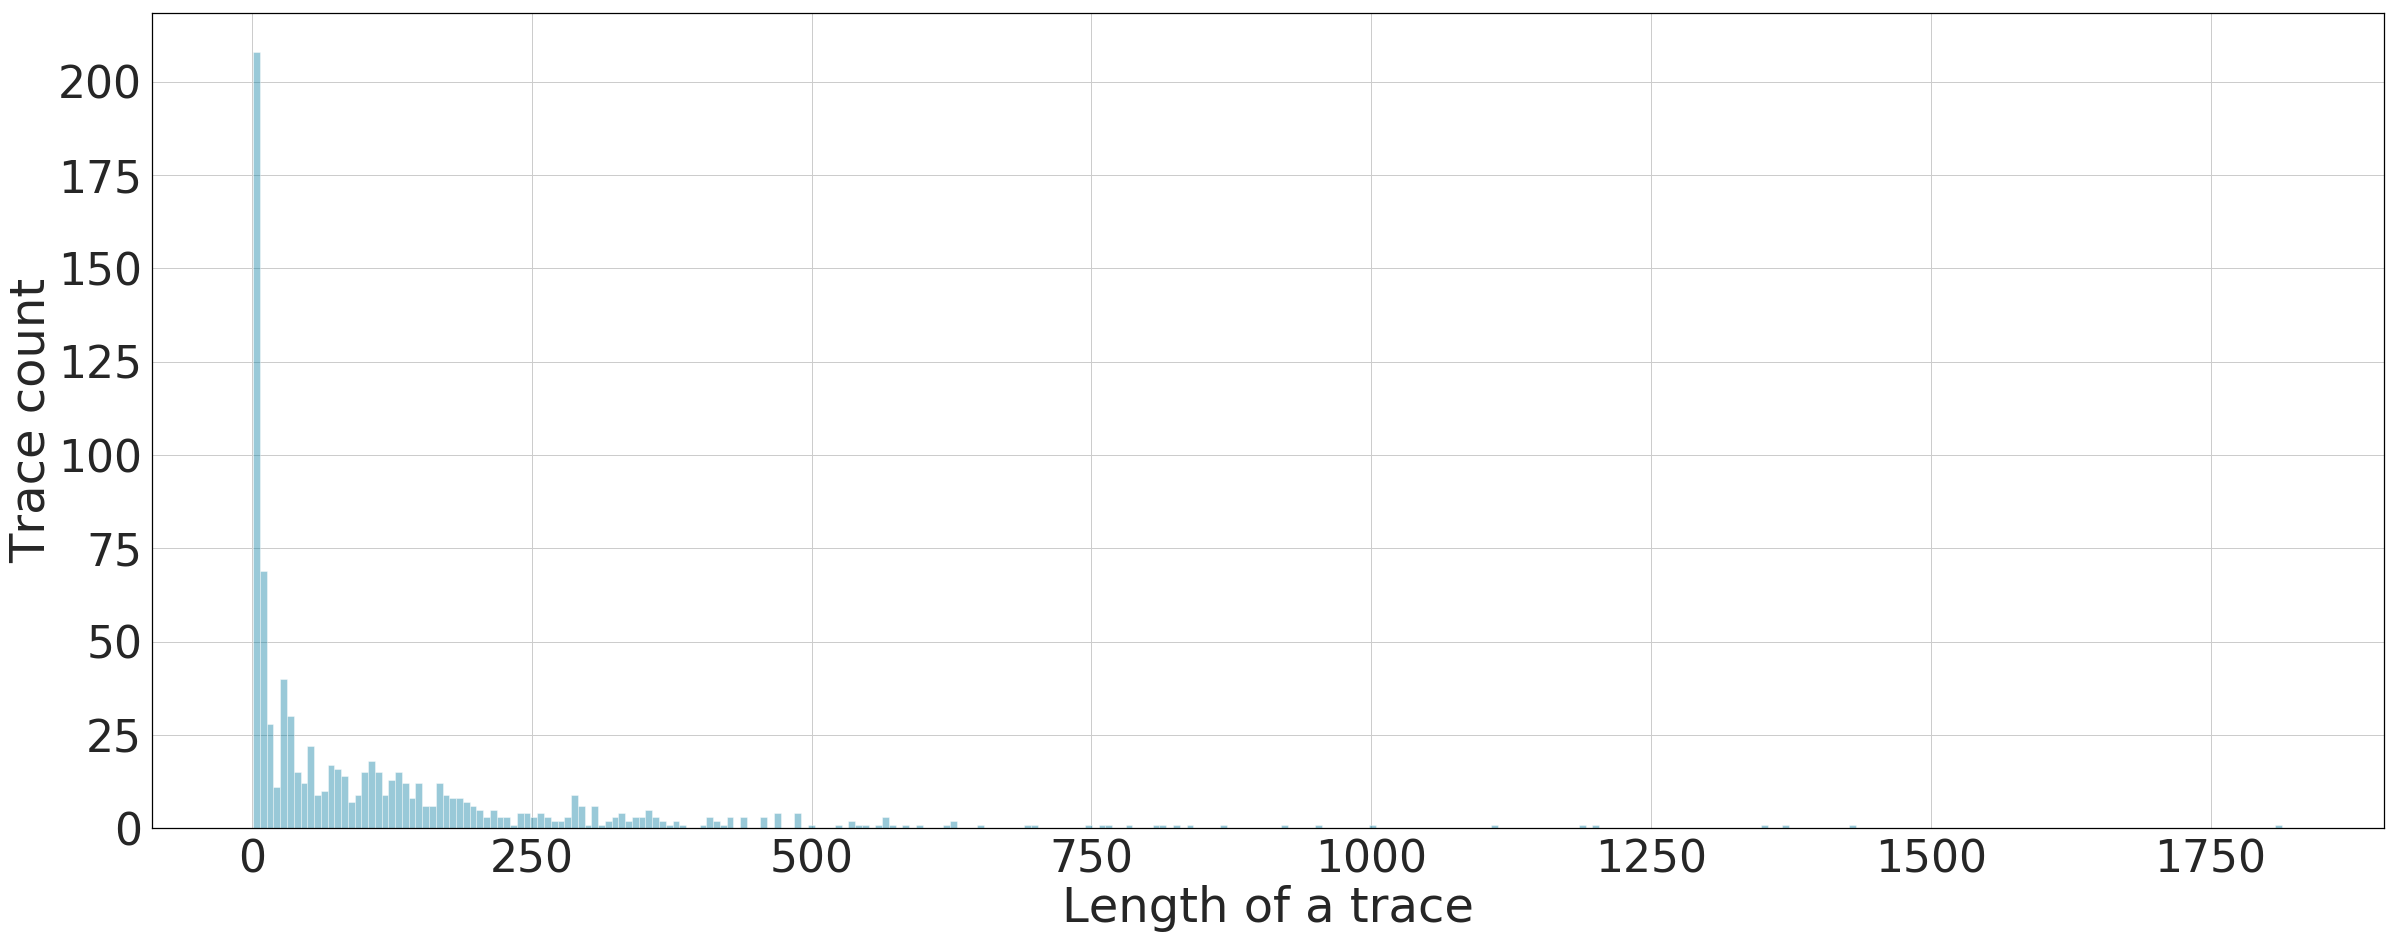
\includegraphics[width=.9\textwidth]{gfx/frequency-distribution.png}
    \caption{Distribution of trace lengths in the BPIC2011 training set.}
    \label{fig:bpic2011-length-distribution}
\end{figure}

Third, there is the possibility of padding the number of time-steps in a sequence to the same length and using a Masking layer to then filter out the padded values during training~\cite{web:keras}. The padding length is dictated by the maximum trace length and may incur a large memory overhead if it is a large outlier value.

Fourth and finally, there is also the possibility to split the trace into samples by sliding a window along it. This results in $l-w+1$ samples for a trace of length $l$ and a window width $w$. Taking \autoref{tab:sliding-window} in \autoref{sec:background:feature-engineering} as an example, the window would be two timesteps wide. While this approach solves the problem of unequal sample lengths and facilitates batch construction, the model can only use a maximum of $w$ timesteps per sample for training, thus losing potential long-term dependencies. As both Evermann et al.~\cite{evermann2016} and Schönig et al.~\cite{schoenig2018} use this format and it directly opposes the findings of Klinkmüller et al.~\cite{klinkmuller2018reliablemonitoring}, we investigate it. Furthermore, we believe that a windowed training data format misses out on LSTM potential.\\

The four batching strategies are labelled in the order of the preceding description for easier reference in the next chapter where they are evaluated:
\begin{itemize}
    \item\textbf{Individual}: One trace per batch
    \item\textbf{Grouped}: Same-length traces in one batch
    \item\textbf{Padded}: Padded-to-length traces
    \item\textbf{Windowed}: Windowed samples, as used by Evermann and Schönig
\end{itemize}

\section{A next-event predictive model training framework}
\label{sec:contrib:training-framework}
We realize that making different process prediction approaches comparable is not only a technical but also a data-related challenge - no established benchmarking datasets for Predictive Process Monitoring exist yet.
To mitigate this situation, we designed the software framework that helped us compare the sixteen total model-batching-strategy combinations on a variety of datasets in an extensible way. Doing so enables future researchers to build upon this framework and publish performance numbers from models that were trained on the same data.\\

\begin{figure}
    \centering
    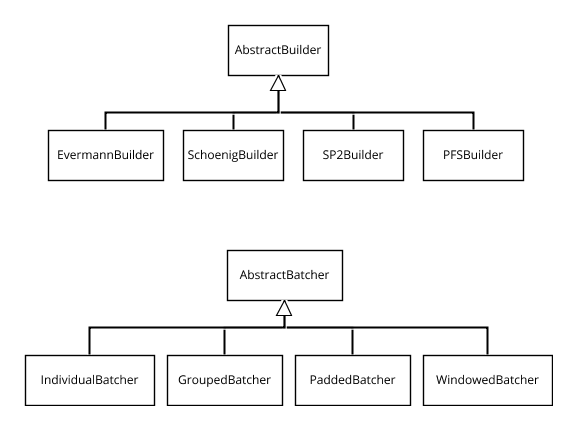
\includegraphics[width=\textwidth]{gfx/training-framework-classes.png}
    \caption{A Unified Modeling Language (UML) diagram of the abstract base class inheritance structure of Builders and Batchers.}
    \label{fig:trainig-framework-classes}
\end{figure}

The proposed framework distinguishes between two important concepts: Builders and Batchers. As \autoref{fig:trainig-framework-classes} shows, these two basic concepts are introduced as abstract base classes from which the actual model and batching strategy implementations are derived.\\

\noindent\textbf{Builders} construct Keras models and also define the structure of the training and test data. This is important as models may not only have one input layer, but two or more. These pre-formatted data sets are not structured into batches yet. One such Builder is implemented for every model type by inheriting from the abstract base class \verb=AbstractBuilder=.

\noindent\textbf{Batchers} take the pre-formatted data sets and structure them into batches. For each batching strategy, one class inherits from the abstract base class \verb=AbstractBuilder=.\\

A frontend named \verb=model_runner= ties these two concepts together with training logic and provides a basic command-line interface for directing the training process to a specific GPU, and defining the output directory for the model and performance files and the location of the input files. It allows for flexibly training a model with a specific Builder and a specific Batcher.\\

The inheritance structure allows all classes to implement the same interfaces, which make the interaction in \autoref{fig:} possible. This exchange enables the flexibility that this framework provides.\\

With the help of this framework, future researchers only need to subclass \verb=AbstractBuilder=, and can directly evaluate the model performance on any given dataset without having to implement the whole training environment. By simply sharing their Builder and Batcher implementations, it will be much easier for other researchers to reproduce findings. The framework and detailed documentation is hosted under \href{https://github.com/flxw/ppm-tf}{flxw/ppm-tf}
\todo[inline]{Create this repository anlong with its documentation and usage instructions.}

\begin{figure}
\centering
\begin{verbatim}
usage: model_runner.py [-h] [--gpu GPU]
                       [--output OUTPUT]
                       {evermann,schoenig,sp2,pfs}
                       {padded,grouped,individual,windowed}
                       datapath

The network training framework script for Felix Wolff's master's thesis!

positional arguments:
  {evermann,schoenig,sp2,pfs}
                        Which type of model to train.
  {padded,grouped,individual,windowed}
                        Which mode to use for feeding
                        the data into the model.
  datapath              Path of dataset to use for training.

optional arguments:
  -h, --help            show this help message and exit
  --gpu GPU             CUDA ID of which GPU the model
                        should be placed on to
  --output OUTPUT       Target directory to put model
                        and training statistics
\end{verbatim}
\caption{The \texttt{model\_runner} command-line frontend for the training framework.}
\label{fig:framework-frontend}
\end{figure}
